\documentclass{beamer}
\usepackage{beamerthemeSingapore}
\usepackage{amsfonts,amsmath,amssymb}
\usepackage{graphics}
\usepackage{graphicx}
\usepackage{colortbl}
\usepackage{wasysym}
\usepackage{verbatim}
\usepackage{hyperref}
\hypersetup{colorlinks=true}
\usepackage{Sweave}

\title{xstatR: an Environment for Running\\ 
R and XLISP-STAT in Docker Containers\\  
UseR! 2019}

\author{E. James Harner and Jun Tan}
\institute[West Virginia University]{
  West Virginia University\\
  Rc$^2$ai
}

\date[]{July, 2019}

\subject{}

% Delete this, if you do not want the table of contents to pop up at
% the beginning of each subsection:
\AtBeginSubsection[]
{
  \begin{frame}<beamer>
    \frametitle{Outline}
    \tableofcontents[currentsection,currentsubsection]
  \end{frame}
}

% If you wish to uncover everything in a step-wise fashion, uncomment
% the following command: 
%\beamerdefaultoverlayspecification{<+->}

\begin{document}
\Sconcordance{concordance:xstatRTalk.tex:xstatRTalk.Rnw:%
1 341 1}


\begin{frame}
  \titlepage
\end{frame}

\begin{frame}
  \frametitle{Outline}
  \tableofcontents
  % You might wish to add the option [pausesections]
\end{frame}

\section{Introduction}

\begin{frame}
\frametitle{Why XLISP-STAT?}
\begin{itemize}
	\item 
\end{itemize}
\end{frame}

\begin{frame}
\frametitle{Integrating R and XLisp-Stat}

Two dockerized environment have been created for integrating R and XLisp-Stat.
\begin{description}
	\item[xstatR] for embedding R into XLisp-Stat using the R dynamic library
	\item[RXLisp] for embedding XLisp-Stat into R using the XLisp-Stat dynamic library
\end{description}
\vspace{0.5 cm}
\texttt{xstatR} was originally presented by Jim Harner with programming support by Jun Tan in the 2009 \href{https://www.r-project.org/DSC-2009/}{Directions in Statistical Computing (DSC) Workshop} held in Copenhagen.\\
\vspace{0.5 cm}
\href{http://www.omegahat.net/RXLisp/index.html}{RXLisp} was developed by Duncan Temple Lang in 2002.
\end{frame}

\begin{frame}
\frametitle{xstatR: Linking via the R dynamic library}

\texttt{xstatR} is designed for the user who wants the full XLisp-Stat environment with extensions for advanced dynamic graphics and a full R environment both accessible by a command-line interface with X11 support.

\begin{itemize}
	\item Allows for a natural interface for software written in C
	\item Calls R directly
	\item Does not depend on other software, except for R
	\item Needs no setup or configuration
	\item Compile R with the --enable-R-shlib option
	\item Recompile xlispstat after upgrading R (if necessary)
\end{itemize}
\end{frame}

\begin{frame}
\frametitle{RXLisp: Linking via the XLisp-Stat dynamic library}
\texttt{RXLisp} is designed for an R user who wants access to the dynamic graphics of XLisp-Stat using the syntax of R.
\begin{itemize}
	\item Loads XLisp into R as an R package
	\item Implements a subset of XLisp-Stat, e.g., callbacks not currently supported
	\item Allows an R interface to XLisp-Stat (with an optional XLisp interface)
	\item Requires little knowledge of XLisp-Stat except the functions of interest
\end{itemize}
\end{frame}

\begin{frame}
\frametitle{What is Docker?}

\href{https://www.docker.com/what-docker\#/container-platform}{Docker containers} provides a platform for running \texttt{xstatR} and \texttt{RXLisp}.\\
\vspace{0.5 cm}
The two principal Docker entities are:
\begin{description}
	\item[Image:] an executable package that includes everything needed to run an application 
	\item[Container:] a runtime instance of an image
\end{description}
The image contains the code, configuration files, environmental variables, libraries, and the runtime. A container is an image with state, i.e., a user process.\\
\vspace{0.5 cm}
The \texttt{xstatR} and \texttt{RXLisp} images provide complete, immutable solutions for embedding R in XLisp-Stat or embedding XLisp-Stat in R, respectively.

\end{frame}

\section{xstatR Architecture}

\begin{frame}
\frametitle{A Layered Structure}
\begin{itemize}
	\item C/R Interface
	\item Low level Lisp/R API
	\item High level Lisp/R API
\end{itemize}
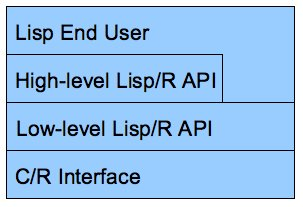
\includegraphics{layers.jpg}
\end{frame}

\begin{frame}
\frametitle{C/R Interface}
\begin{itemize}
	\item The C/R interface is a thin wrapper of the embedded R API.
	\item The C/R interface avoids name conflicts between xlispstat and R
	\item R functions are mapped to C-based R interface macros/functions in xlispstat
	\item The C/R layer is invisible to users of xlispstat
\end{itemize}
\end{frame}

\begin{frame}
\frametitle{Low Level Lisp/R API}
\begin{itemize}
	\item Developed in C for communicating with the external C interface in R
	\item Provides basic functions for allowing the Lisp user to access R
	\item Requires the user to take care of details, e.g., data synchronization between Lisp and R
	\item Designed for developers and advanced users
	\item Used as a platform for xlispstat packages, e.g., xstatR, that require the flexible use of R 
\end{itemize}
\end{frame}

\begin{frame}
\frametitle{High Level Lisp/R API}
\begin{itemize}
	\item Developed in Lisp
	\item Communicates with the low-level C macros/functions
	\item Provides convenient functions based on the embedded R environment
	\item Hides the embedded R environment from the user
	\item Is customizable and extendible, e.g., the user can customize the mapping between an R object and a Lisp object 
\end{itemize}
\end{frame}

\section{Data mapping}

\begin{frame}
\frametitle{Data type mapping}
\begin{itemize}
	\item Data type mapping needs to be dealt with in bridging/interface software
	\item One-to-one mapping is the ideal situation
	\item Due to the rich data structures in Lisp and R and their flexibility, no such mapping exists
\end{itemize}
\end{frame}

\begin{frame}
\frametitle{A possible solution}
\begin{itemize}
	\item Convert simple data types, e.g., vectors of scalers.
	\item Returns a reference to R objects rather than converting complex data types
	\item Depends on the user to retrieve information from the R object references
	\item Used by R interface packages such as JRI and RServe
\end{itemize}
\end{frame}

\begin{frame}
\frametitle{Problems of this method}
\begin{itemize}
	\item R objects need to be locked to avoid garbage collection
	\item User is responsible for releasing R objects
	\item Proper access methods to the object references are needed
\end{itemize}
\end{frame}

\begin{frame}
\frametitle{Our strategy}
\begin{itemize}
	\item Use a generic structure to represent R objects
	\item Copy the data into this structure, ignoring unrecognized components
	\item Unlock the R object by default after all information is copied
	\item Assign R objects to variable names to retain them in memory, if persistence is needed
\end{itemize}
\end{frame}

\begin{frame}
\frametitle{The generic structure representing R objects}
\begin{itemize}
	\item A list of length one or three
	\item The first element is the data part
	\item The second and third elements, for R objects with attributes, are the attribute names and the attribute values
	\item Attribute name list is a list of strings
	\item Attribute value list provides the corresponding values of the named attributes
	\item Data part is either an array of scalars/strings, etc., or (recursively) a list of generic structures
\end{itemize}
\end{frame}

\begin{frame}
\frametitle{Current Implementation}
\begin{itemize}
	\item Many complicated structures are (currently) copied without special handling, e.g., \texttt{lm} objects.
	\item This structure is not convenient for direct use.
	\item The generic structure is a good foundation for building highly flexible conversions to meet users' needs, e.g., as has been implemented for data frames.
\end{itemize}
\end{frame}

\section{Main functions}

\begin{frame}
\frametitle{Low Level C Functions}
\begin{itemize}
	\item \texttt{(callR "\emph{R statement}")}\\
	Parse and evaluate an R statement. The evaluation result will be copied into a generic structure and returned to the user.
	\item \texttt{(saveToR "\emph{rName}", \emph{lispObj})}\\
	Save the value of \texttt{lispObj} into the embedded R environment (the value has to be encoded into the 	generic structure).
\end{itemize}
\end{frame}

\begin{frame}
\frametitle{Examples}
\texttt{
\\
(setf y-list (callR "rnorm(50)")) \\
(setf y (first y-list)) \\
(histogram y) \\
(saveToR "y" y-list)
}
\end{frame}

\begin{frame}
\frametitle{High level functions: converting R objects}
\begin{itemize}
	\item A prototype, \texttt{Rengine-proto}, was built to ease the process of calling R.
	\item  \texttt{Rengine-proto} directly supports the xstatR package, but can be used by any xlispstat package.
	\item The user can determine how to convert an R object based on its class name, dimension, etc. 
	\item  \texttt{Rengine-proto} currently includes loading data from R, saving an xstatR dataset to an R data frame, etc.
\end{itemize}
\end{frame}

\begin{frame}
\frametitle{List of major methods}
\begin{itemize}
	\item \texttt{(send R :call \emph{"statement"} \&key \emph{asis})}\\
	Parse and evaluate a R statement.\\
	\texttt{\emph{asis}} is a boolean value indicating whether to bypass the conversion process or not
	\item \texttt{(send R :save \emph{"rName"} \emph{lispObj}\\ 
	\&key \emph{attr attrNames})}\\
	Save a lisp object to R. Attributes and names can be attached
	\item \texttt{(send R :save-dataset \emph{"rName"} \emph{lispObj}\\ 
	\&key \emph{cols rows})}\\
	Save a dataset or part of a dataset as data frame in R
\end{itemize}
\end{frame}

\begin{frame}
\frametitle{Examples}
\texttt{
\\
(setf iris (send R :data "iris")) \\
(send R :save-dataset "iris.data" iris \\
	:cols '(SEPAL.LENGTH SEPAL.WIDTH) \\
	:rows (iseq 1 10)) \\
(send R :call "ls()") \\
(setf x (send R :call "iris.data")) 
}
\end{frame}

\section{xstatR}

\begin{frame}
\frametitle{The xstatR package}
\begin{itemize}
	\item A lisp package used for dynamic graphics, data modeling, and multivariate analysis
	\item Dataset objects are defined in terms of observation objects
	\item Virtual datasets are constructed to encapsulate derived variables from model or other statistical objects
	\item Observations are objects viewable in different graphs
	\item Point state, color, and symbol are properties of the observation
	\item Changes in an observation value or property is immediately updated in its linked views
	\item R acts as a computational engine using the Lisp/R bridge
\end{itemize}
\end{frame}

\begin{frame}
\frametitle{Partial Overview}
\begin{center}
	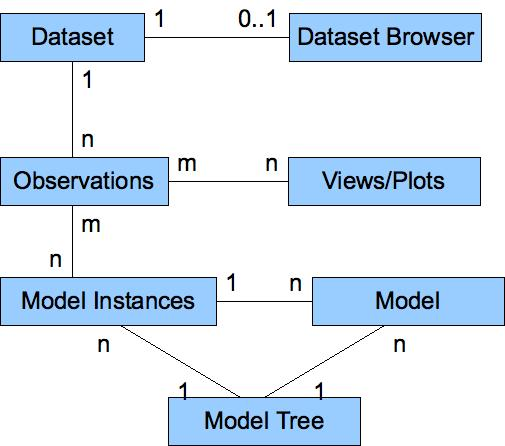
\includegraphics[width=0.6\textwidth]{xstatR.jpg}
\end{center}
\end{frame}

\begin{frame}
\frametitle{Linked plots}
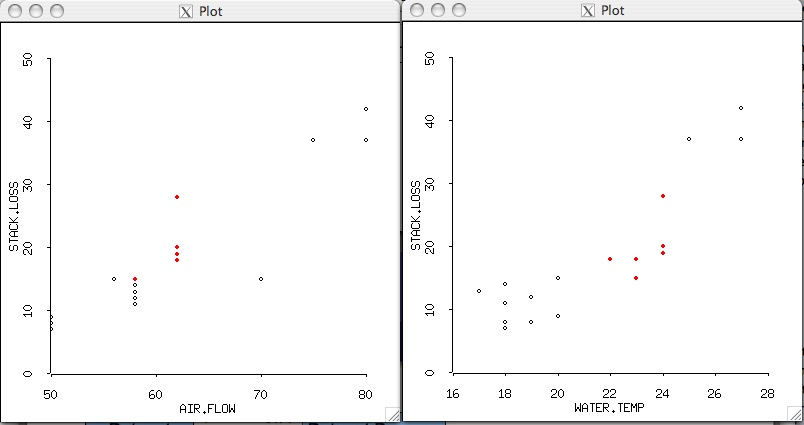
\includegraphics[width=\textwidth]{linkedPlots.jpg}
\end{frame}

\begin{frame}
\frametitle{Modeling Tree}
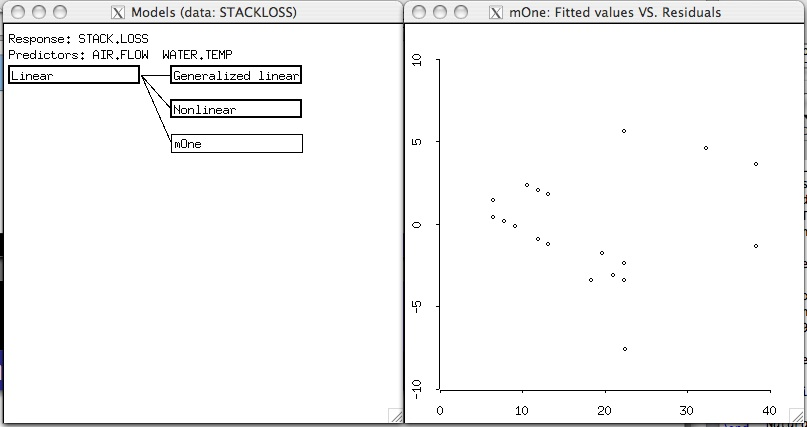
\includegraphics[width=\textwidth]{modeling.jpg}
\end{frame}

\begin{frame}
\frametitle{More about virtual datasets for models}
\begin{itemize}
	\item Models generate derived variables from the original model variables.
	\item The newly generated data often need to be combined with the original dataset, e.g., to plot residuals against a predictor.
	\item SAS/JMP add (optionally) derived variables from models to the same dataset and the user soon loses track of which derived variables go with which model.
	\item R generates (optionally) named model and summary objects and the user soon loses track of the underlying models/summaries.
	\item Virtual datasets combined with tree-based model visualizations provide a solution.
\end{itemize}
\end{frame}

\begin{frame}
\frametitle{Currently working on...}
\begin{itemize}
	\item Virtual datasets combine the ``variables'' in a dataset with the ``derived variables'' from a model object
	\item The dataset browser shows the virtual dataset by clicking on the statistical object view, e.g., a model view
	\item Virtual datasets support linking, e.g., for  model diagnostic plots
	\item Virtual model datasets combined with a model tree recursively allow model comparisons 
\end{itemize}
\end{frame}

\section{RXLisp Architecture}

\end{document}


